\documentclass[12pt, a4paper]{article}
\usepackage{fontspec}
  \defaultfontfeatures{Mapping=tex-text}
  \setromanfont [Ligatures={Common}]{Linux Libertine O}
\usepackage{sectsty}
  \sectionfont{\upshape\large}
  \subsectionfont{\mdseries\scshape\normalsize} 
  \subsubsectionfont{\mdseries\upshape\large}
\usepackage{tabularx}
\usepackage[usenames,dvipsnames,svgnames,table]{xcolor}
  \definecolor{tnzbrown}{HTML}{503E32}
  \definecolor{tnzgreen}{HTML}{118A47}
\PassOptionsToPackage{hyphens}{url}\usepackage{hyperref}
  \hypersetup{colorlinks=true,linkcolor=tnzgreen,urlcolor=tnzgreen}
\usepackage[font={color=tnzbrown}]{caption}

\title{\textbf{A No-install Solution to Enabling/Disabling the Titlebar in Xfce}}
\author{Joaquim Baeta}
\date{July 16, 2014\\ \normalsize \emph{(\textbf{Updated} \today)}}

\begin{document}
\maketitle

\noindent \emph{\textbf{Update, 2015-05-20:} As of Xfce 4.12\footnote{Xfce development team, ``Xfce 4.12 released," Xfce, February 28, 2015, \url{http://www.xfce.org/about/news/?post=1425081600}}, this solution works without the need for plugins. It also works out of the box in Xubuntu 15.04, but may not in older versions unless you've updated to Xfce 4.12.\footnote{Andrew, ``Install Xfce 4.12 In Xubuntu 14.04 Or 14.10 Via PPA," \emph{WebUpd8}, March 03, 2015, \url{http://www.webupd8.org/2015/03/install-xfce-412-in-xubuntu-1404-or.html}}}\\

\noindent I found a little quirk when I upgraded to Xubuntu 14.04: the titlebar no longer appeared when I maximised a window. Because I habitually exploit the titlebar, this was a cumbersome change (or bug). Fortunately, I found out how to reverse it quickly enough.

Initially, I thought the solution was obvious enough to go without a mention. A recent article by Andrew on \emph{WebUpd8}\footnote{Andrew, ``Xubuntu: How To Put Maximized Windows Buttons And Title On The Panel," \emph{WebUpd8}, July 14, 2014,  \url{http://www.webupd8.org/2014/07/xubuntu-how-to-put-maximized-windows.html}.}, though, introduced the intriguing xfce4-windowck-plugin\footnote{Alessio Piccoli and Cédric Leporcq, Xfce, accessed July 16, 2014, \url{http://goodies.xfce.org/projects/panel-plugins/xfce4-windowck-plugin}.} by Alessio Piccoli and Cédric Leporcq. It's a set of two plugins enabling you to place a maximised window's title in the panel, along with the window's buttons. If you install xfce4-windowck-plugin, you likely want to disable the titlebar to avoid redundancy. Andrew and xfce4-windowck-plugin's developers suggest installing the external program Maximus or a patch for xfwm4\footnote{cedl38, xfwm4-titleless, accessed July 17, 2014, \url{https://github.com/cedl38/xfwm4-titleless}}.

My solution is simpler and doesn't require you to download or install anything.

\section*{Comparison of maximised windows with and without the titlebar}

For reference, Figure~\ref{fig1} shows a maximised window with the titlebar, while Figure~\ref{fig2} shows it without.

\begin{figure}[!h]
  \centering
  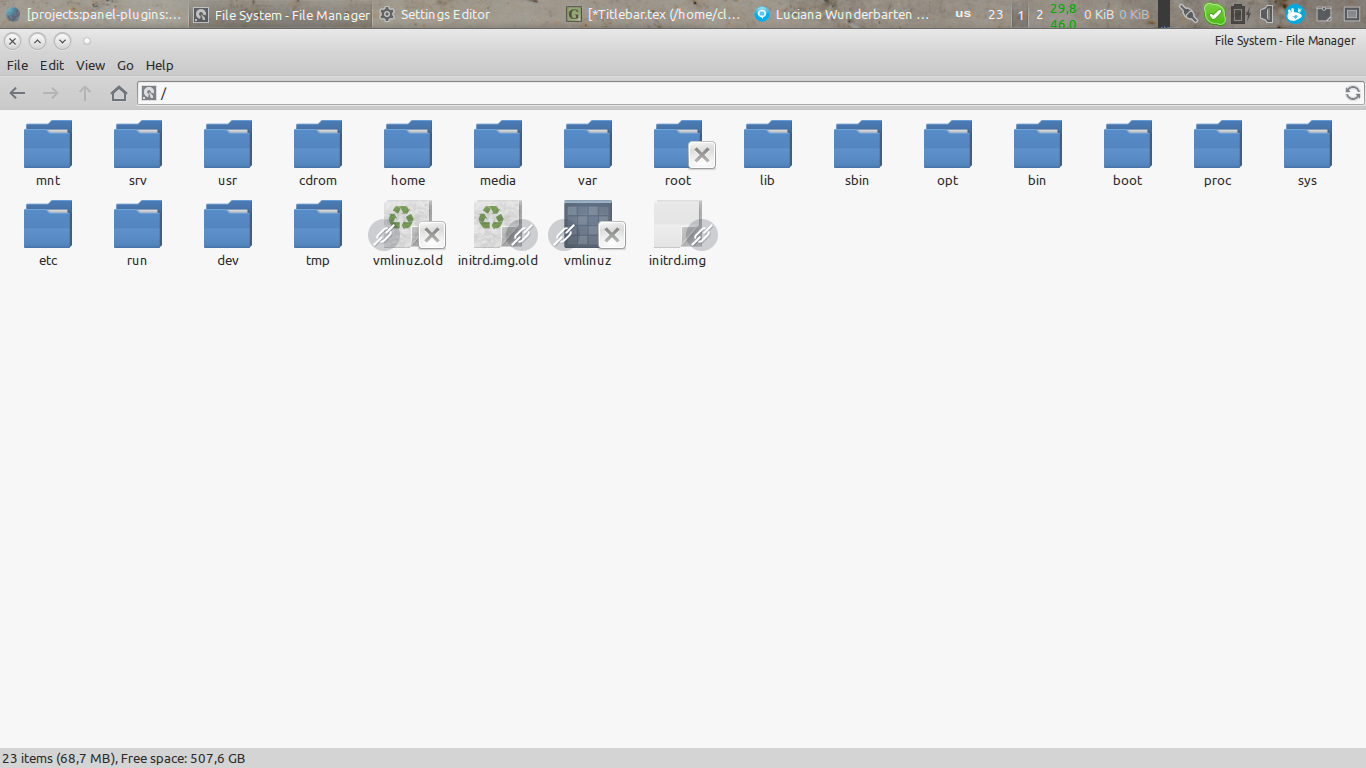
\includegraphics[width=1\textwidth]{imgs/1xfcewithtitlebar.png}
  \caption{Maximised window in Xfce with the titlebar.}
  \label{fig1}
\end{figure}

\begin{figure}[!h]
  \centering
  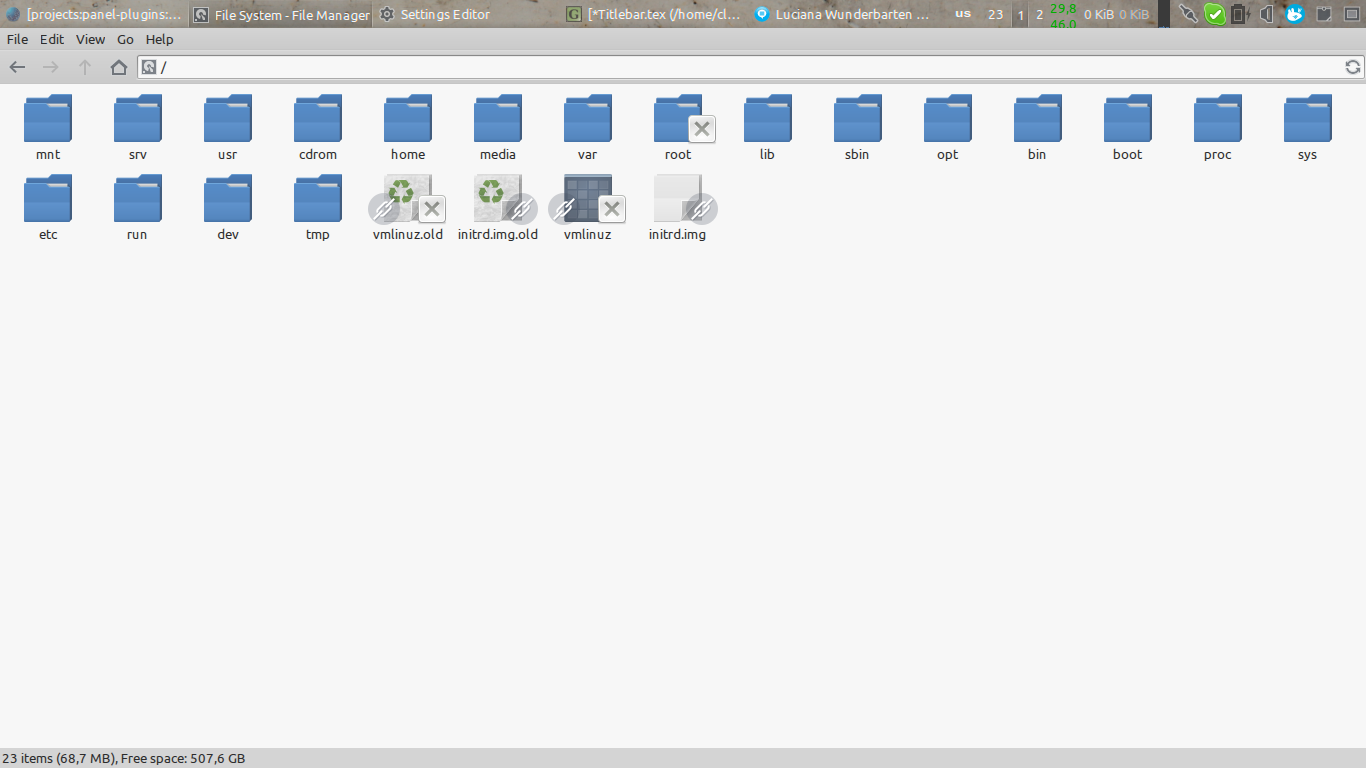
\includegraphics[width=1\textwidth]{imgs/2xfcewithouttitlebar.png}
  \caption{Maximised window in Xfce without the titlebar.}
  \label{fig2}
\end{figure}

\section*{Solution}

\emph{You can skip Steps 1 and 2 by typing ``xfce4-settings-editor" in the Terminal and jumping straight to Step 3. Otherwise, start from Step 1.}\\

\noindent \textbf{Step 1:}\\

\noindent Open the Settings Manager (Figure~\ref{fig3}). In Xubuntu 14.04 onward, you can do this using Whisker Menu, or the applications menu in earlier versions. Alternatively, you can also open it through the Terminal, using the command ``xfce4-settings-manager".

\begin{figure}[h]
  \centering
  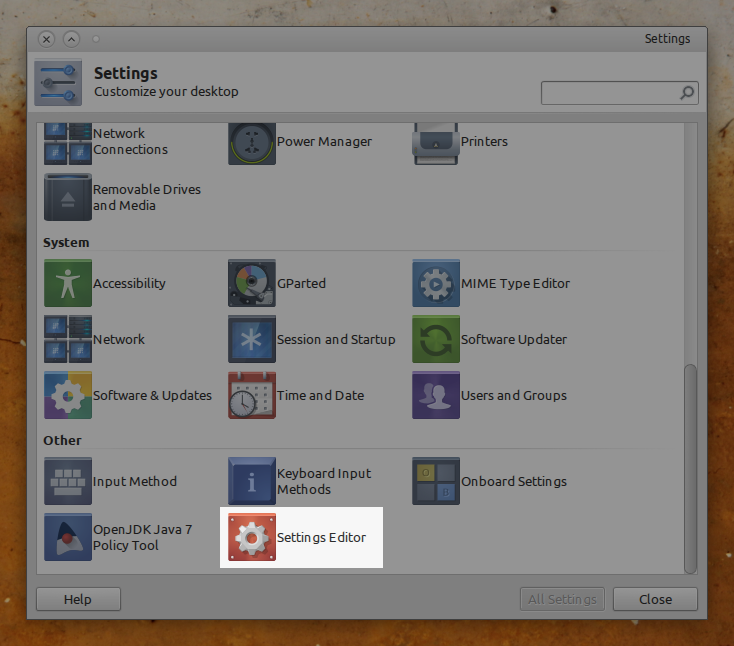
\includegraphics[width=1\textwidth]{imgs/3settingsmanager.png}
  \caption{Location of Settings Editor in Settings Manager.}
  \label{fig3}
\end{figure}

\newpage
\noindent \textbf{Step 2:}\\

\noindent Scroll to the bottom of Settings Manager and open Settings Editor (Figure~\ref{fig3}). You can also open it using the Terminal with the command ``xfce4-settings-editor".\\

\noindent \textbf{Step 3:}\\

\noindent On the left tab, scroll to the bottom and look for ``xfwm4" (Figure~\ref{fig4}). Click it and now on the right side scroll down to find ``titleless\_maximize" (Figure~\ref{fig5}).

\begin{figure}[h]
  \centering
  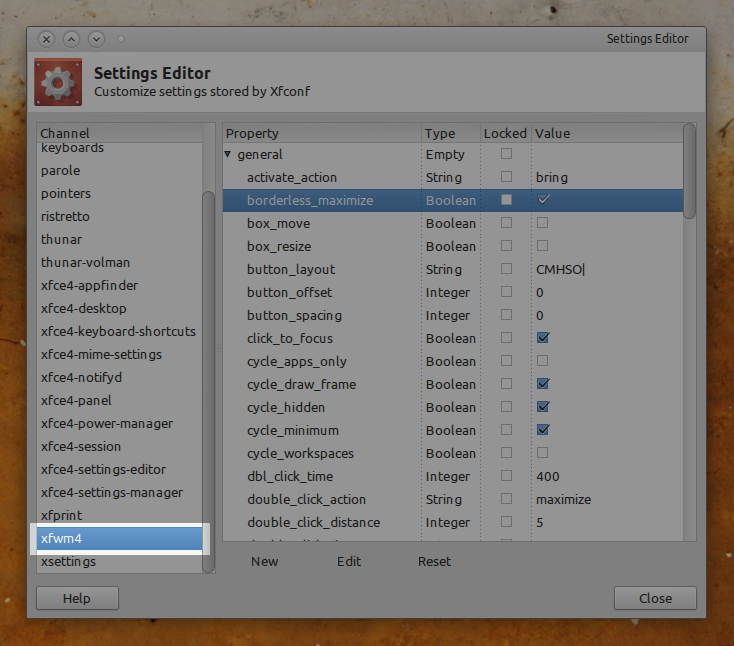
\includegraphics[width=1\textwidth]{imgs/4settingseditor.png}
  \caption{Location of ``xfwm4" in Settings Editor.}
  \label{fig4}
\end{figure}

\begin{figure}[h]
  \centering
  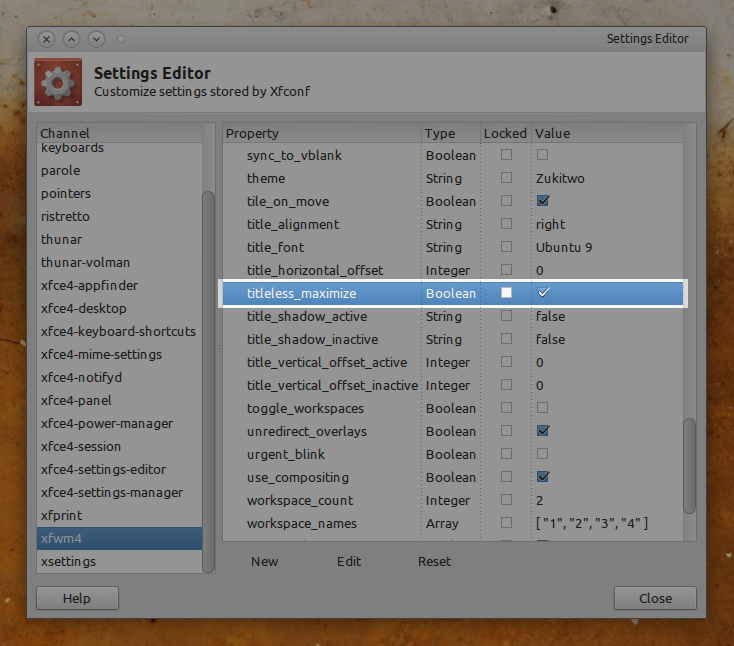
\includegraphics[width=1\textwidth]{imgs/5titlelessmaximise.png}
  \caption{Location of ``titleless\_maximize" in Settings Editor. The ticked value in the right-most column shows that the titlebar is currently hidden when maximised.}
  \label{fig5}
\end{figure}

\noindent \textbf{Step 4:}\\

\noindent Now the part that actually fixes it. In the \emph{Value} column, ``titleless\_maximize" will either be blank or ticked. If it is blank, then Xfce will display the titlebar when windows are maximised; if it is ticked, it will not. (Yes, it's a bit counter-intuitive.) Simply tick or untick this value to choose your preference.\\

\noindent That's it!

\section*{Bonus solution}

Settings Editor has a surprising amount of power if you're willing to experiment. Related to hiding the titlebar is hiding window borders, as well. Follow the same steps as above, but look for ``borderless\_maximize" instead. 

As Figure~\ref{fig6} shows, borderless\_maximize is currently enabled. This means that when the window is maximised, it takes up the entire screen (save for the panel), instead creating a larger version of the window that merely goes to the edges. \\

\noindent \textbf{Note:} If titleless\_maximize is enabled and you disable borderless\_maximize, the latter will override the former; i.e. both the borders \emph{and} the titlebar will be displayed. This is because the titlebar is considered to be part of the window border.

\begin{figure}[h]
  \centering
  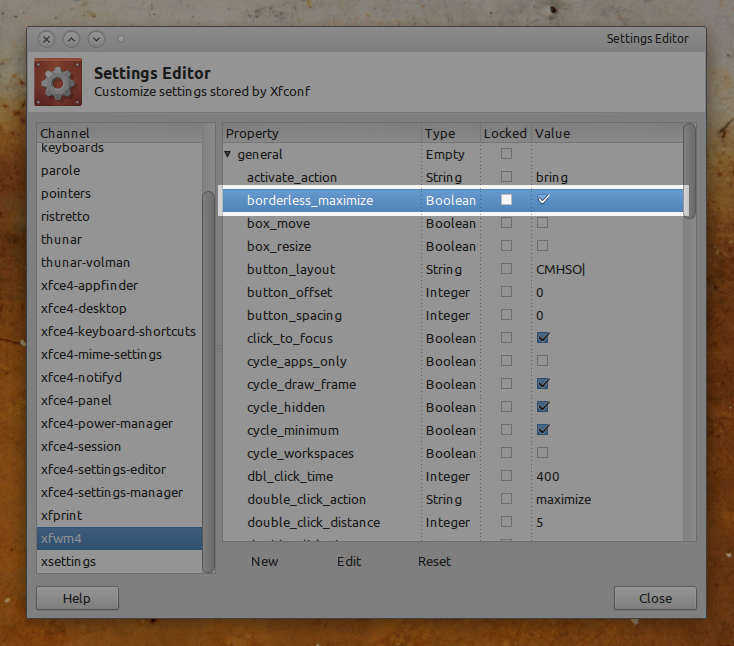
\includegraphics[width=1\textwidth]{imgs/6borderlessmaximise.png}
  \caption{Location of ``borderless\_maximize" in Settings Editor.}
  \label{fig6}
\end{figure}

\section*{TL;DR version}

\textbf{1) Open Settings Editor.\\
2) Under ``xfwm4", look for ``titleless\_maximize".\\
3) Tick to remove titlebar; untick to return titlebar.}\\

\vspace{5cm}
\hrule
\noindent \center \emph{Read online at: \url{http://thenumberzero.blogspot.com/2014/07/a-no-install-solution-to.html}\\
\textbf{Version} 1.2; \textbf{last edited} 2015-05-20\\
\textbf{License:} Creative Commons Attribution-ShareAlike 4.0 International\\
\textbf{Tested OS:} Xubuntu 14.04--15.04;\\ \textbf{Xfce version:} 4.12.1-1; \textbf{xfwm4 version:} 4.12.1-1ubuntu1\\ \textbf{Theme:} Zukitwo; \textbf{icon theme:} Evolvere Blue Folders Dark fallback}
\vspace{1em}
\hrule



\end{document}
